\pdfbookmark{\tth Application}{ttH_dilep application}
\chapter{\tth Application}
\label{Application}

The CERN computational resources, the Worldwide LHC Computing Grid, are organized in a hierarchy divided in 4 tiers. Each tier is made by one or more computing centers and each tier has a set of specific tasks and services to perform. The objective of the whole grid is to store, filter and analyse all the data gathered at the LHC.

The Tier-0 is the data center located at CERN. It provides 20\% of the total grid computing capacity, and its objective is to store and reconstruct the raw data gathered at the detectors in the LHC into meaningful information, usable by the remaining tiers. This tier distributes the raw data and the reconstructed output by the 11 Tier-1 computational centers, spread among the different countries that are part of CERN.

Tier-1 computational centers are responsible for storing a portion of the raw and reconstructed data and provide support to the grid 24/7. In this tier, the reconstructed data suffers more reprocessing, in order to refine it by filtering only relevante information and reducing the size of the data that is then transferred to the Tier-2 computational centers. This tier also stores the outputs of the simulations performed at Tier-2. The Tier-0 center is connected to the 11 Tier-1 centers by high bandwidth optical fiber links, which consists of the LHC Optical Private Network.

There are around 140 Tier-2 computational centers around the world. Their main purpose is to perform Monte-Carlo simulations with the data received from the Tier-1 centers, but also perform a portion of the events reconstructions. The Tier-3 centers range from university clusters to small personnal computers, and they perform most of the events reconstruction and final data analysis.

The LIP research group developed the \tth application to solve the problem presented in section \ref{Motivation}, and it fits in the Tier-3 hierarchy level of event reconstruction and analysis applications. Its name derived from the problem it was design to solve: the tt is relative to the kinematical reconstruction of the two Top Quarks, the \ttbar system, resultant from a head-on particle collision; the H is relative to the Higgs boson reconstruction; the dilep is the name of the routine responsable for the kinematical reconstruction, and it needs two leptons (di-lep) as input.

The application has two main dependencies. The first, and most important, is on the ROOT \ref{CERN:ROOT} object oriented framework, developed at CERN, only available in C++. This framework provides a set of funcionalities oriented for handling, analyzing and displaying results for large amounts of data. It has capabilities of reading and storing data in the standard formats accepted by all the tiers centers, classes for representing physics information, mathematical routines, pseudorandom number generators, histograming, curve fitting minimization and visualization methods. It was originally designed and currently developed mostly by physicists with little knowledge on computer science. This results in a framework that has much room for improvement through a code restructuration in several routines, mostly related to auxiliary functionality, rather than visualization and data storage. Some of the mathematical routines implemented could be replaced by dependencies on other much more stable and faster libraries, such as BLAS \ref{BLAS} or MKL \ref{MKL}. There is an extension to ROOT, the Parallel ROOT Facility (PROOF) \ref{CERN:PROOF}, for parallelization of the work in distributed memory systems, which is not the focus of this thesis work. There is no support nor existing routines parallelized for shared memory systems, which could be made but would require restructuration of portions of the framework code.

The second dependency is on the LipMiniAnalysis library. It is a strip-down version of LipCbrAnalysis, a library developed LIP for in-house use, which provides a skeleton for creating an analysis application. It has the functionality usually necessary in most analysis developed by LIP, and is also prepared for reading a data format different from what is provided by Tier-2, which suffers a filter of the events most likely to provide relevant information after the reconstruction. This library is also not designed for parallelization in shared and distributed memory systems.

\pdfbookmark{Application Flow}{application flow}
\section{Application Flow}
\label{Application:Flow}

This section describes the workflow of the \tth analysis. The callgrind tool from Valgrind \ref{Callgrind} was used to obtain the callgraph of the application, also providing some insight on the time that was being spent in each of its routines. Further analysis of the code itself was necessary to get a better understanding of the application behaviour. In figure \ref{fig:CallgraphOriginal} is presented the callgraph of \tth for 128 variations per combination.

\begin{figure}[!htp]
	\begin{center}
		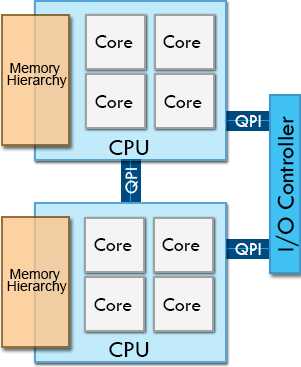
\includegraphics[scale=0.5]{../../common/img/numa_qpi.png}
		\caption{Schematic representation of a NUMA system with QPI interface.}
		\label{fig:CallgraphOriginal}
	\end{center}
\end{figure}

The \ttLoop is the main method of the application. Its purpose is to iterate through all events in the input file and perform 21 filtering and processing tasks (known as cuts) to each event. The most evident problem with the application, inherited from the LipMiniAnalysis library, is the non existence of a data structure on memory holding the events to process. Each input file has around 1 GByte that makes perfectly possible to be stored on RAM memory. However, for each event its information is read from the file and loaded to hundreds of global variables and then it is submited through the cuts. If all the events were read at once, it would be possible to take advantage of the higher bandwidth of sequential reads to the hard drive. Even the overhead of creating such data structure for the events would be compensated by the faster acesses and possibility of easier parallelization of the analysis at the event level, since the events have no dependencies between them.

Every method starting with a capital T refers to the ROOT framework. They are only being used for reading the input file and writing the results. The \ttDoCuts method performs the 21 cuts referred above. It is on cut 20 that \ttDilepKinFit is called, which becomes the most time consuming task as the number of variations per combination increases, as seen from table \ref{tab:TempoKinFit}, therefore, the efforts on improving the performance must be focused on this routine.

\begin{table}[!htp]
	\begin{center}
		\begin{tabular}{|c|c|c|c|c|c|c|c|c|c|c|c|}
			\hline
			\textbf{# of variations/combination} & 1 & 2 & 4 & 8 & 16 & 32 & 64 & 128 & 256 & 512 & 1024 \\ \hline
			\textbf{\% of time} & - & - & - & - & - & - & - & - & - & - & - \\ \hline
		\end{tabular}
		\caption{Percentage of the total execution time spent on the \ttDilepKinFit routine for various numbers of variations per combination.}
		\label{tab:TempoKinFit}
	\end{center}
\end{table}

\todo{terminar tabela com \% tempo na ttdilep}

\pdfbookmark{ttDilepKinFit Routine}{ttDilepKinFit routine}
\section{\ttDilepKinFit Routine}
\label{Application:ttDilepKinFit}

This routine has a main loop that calculates and iterates through all the possible combinations of jets and leptons for a given event. It is possible to define the number of variations to perform per combination, resulting in an inner loop. Some of the variables varied are local to the routine but most are global to the application. The kinematical reconstruction is performed inside the loops, for each variation of each combination and its results, as well as the bottom quarks not used, are used later in the Higgs boson reconstruction. A context is created when the combination to process is calculated, and its specific for the respective combination, which is altered by the variations, kinematical and the Higgs boson reconstructions. Each one of the solutions is stored in a vector and after all the combinations are computed, the said vector is iterated and only the best solution is choosen and its relevant data is copied to global variables.

The quality of a solution is dependent on two factors. The first is the accuracy of the kinematical reconstruction, which is measured by the probability of the reconstruction being properly performed, compared to theoretical models. The second is the accuracy of the Higgs boson reconstruction and its calculation is similar to the former. Since the Higgs boson reconstruction uses results of the kinematical reconstruction, namely the neutrinos and remaining bottom quarks, if the latter is faulty, i.e., performed with a low resultant accuracy, the Higgs boson will be poorly reconstructed too. The accuracy of the overall reconstruction of the event, for a given variance of a combination, is given by the probability of the kinematical reconstruction times probability of the Higgs boson reconstruction.

\begin{figure}[!htp]
	\begin{center}
		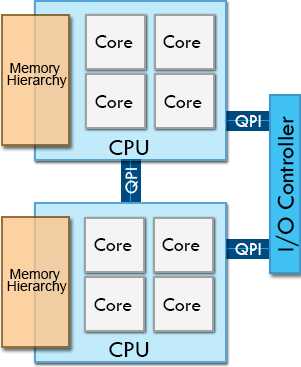
\includegraphics[scale=0.5]{../../common/img/numa_qpi.png}
		\caption{Schematic representation of a NUMA system with QPI interface.}
		\label{fig:CallgraphKinFit}
	\end{center}
\end{figure}

Note that the flow of \ttDilepKinFit may change between combinations, or even variations, within an event. The responsible of that behaviour is the \dilep routine. A certain combination may be capable of being reconstructed, both the \ttbar system and the Higgs boson, but with others the \ttbar system may not be reconstructable, which causes the \ttDilepKinFit flow to stop and process the next combination. This irregularity of the time that takes to process a combination can be problematic to the load balancing of the parallel tasks, as explained in section \ref{Parallelization:Sequential}.

The callgraph for the \ttDilepKinFit for 128 variations per combination is presented in figure \ref{fig:CallgraphKinFit}. The sections of the routine that are most relevant, the variation of the events parameters, the kinematical and Higgs boson reconstructions, are explained in depth in the next subsections.

\pdfbookmark{Variations Routine}{variations routine}
\subsection{Variations Routine}
\label{Application:Variations}

The purpose of the variation is to overcome the experimental resolution of the ATLAS detector, as explained in section \ref{Motivation}.The variation of the parameters of an event, for a given combination of jets and leptons, consists on applying an offset of a given magnitude to the said values. The offset is randomly obtained, using the TRandom3 pseudo-random number generator from ROOT, following a gaussian distribution. The mean value used is 0 and the standard deviation is 2\%, as it is the resolution error of the detector associated to every measurement. The values varied are the momentums of the 2 jets and 2 leptons that make the combination, and consequently their energy is recomputed.

The pseudo-random number generator used by the TRandom3 class is the Mersenne Twister \ref{MersenneTwister}, currently one of the most used generators for applications highly dependable on random numbers. This algorithm produces 32-bit uniformly distributed pseudo-random numbers with a period of $2^{19937}$. It has a relatively heavy state which is an integrant part on the algorithm flow. The generator is thread safe as long as different states are being used in different threads. The state can be shared among the threads but, however, change it must be done sequentially, sequentializing the number generation among the threads. In this case, the number generated by one thread will affect the number generated by the remaining.

\nvidia offers a parallel implementation of the Mersenne Twister for GPUs in the cuRand library \ref{NVIDIA:MersenneTwister}. It uses a precomputed set of 200 parameters, which can also be generated by the user, but offering a smaller period of $2^{11213}$. The pseudo-random number generation and state update is thread safe, up to 256 threads sharing the same state structure, for each block. Two different blocks can safely operate concurrently.

TRandom uses the Acceptance-Complement Ratio algorithm \ref{AcceptanceRandom} for transforming the pseudo-random numbers from an uniform to a gaussian transformation. It is allegely 66\% faster than the Box-Muller transformation \ref{BoxMuller} and similar to the Ziggurat method \ref{Ziggurat}. The cuRand library only offers the Box-Muller transformation with a basic pseudo-random number generator so, to accuratly replicate the results, it is needed to replicate the TRandom gaussian method on GPU using the cuRand implementation of Mersenne Twister.

\pdfbookmark{dilep Routine}{dilep routine}
\subsection{\dilep Routine}
\label{Application:dilep}

The kinematical reconstruction is performed in the \dilep routine. The \ttbar system obeys a set of properties of an theoretical expected model. To reconstruct both of the Top Quarks it is needed to know the characteristics of all resultant particles from their decay. However, since the neutrinos do not react with the detector, and their characteristics are not recorded, it is needed to infer them, using the properties of momentum and energy conservation of the system. Once the neutrinos characteristics are determined, it is possible to reconstruct the Top Quarks.

\dilep analitically solves a system of 6 equations to infer the neutrinos characteristics and then reconstruct the Top Quarks. The routine is dependent on only one class from ROOT, TLorentzVector, making it easy to port to GPU. Executions of \dilep on different inputs are completely independent, since this function does not alter the global state of the \tth analysis.

\pdfbookmark{ttDilepKinFit Routine Computational Analysis}{ttDilepKinFit routine computational analysis}
\subsection{\ttDilepKinFit Routine Computational Analysis}
\label{Application:ttDilepKinFit:Analysis}

\todo{Coisas papi}